\documentclass{plt}
\usetheme{metropolis}           % Use metropolis theme

\title{Runtime Environments}
\author{Ronghui Gu}
\institute{Columbia University}
\date{Spring 2019}
\titlegraphic{
\vspace{220pt}
{\tiny $^*$ Course website: \url{https://www.cs.columbia.edu/~rgu/courses/4115/spring2019}\vspace{-5pt}}\\
{\tiny $^{**}$ These slides are borrowed from Prof. Edwards.}
}

\tikzset{
  byte/.style={fill=gray,minimum height=16pt,minimum width=20pt,text=white},
  hbyte/.style={fill=darkred,minimum height=16pt,minimum width=20pt,text=white},
  bytes/.style={matrix of nodes/.style={
           execute at begin cell=\node\bgroup,
           execute at end cell=\egroup;,
           execute at empty cell={\node [byte] {};}},
           matrix of nodes,
           every node/.style=hbyte},
  every matrix/.style={row sep=2pt,column sep=2pt},
  free/.style={draw,minimum height=16pt},
  used/.style={draw,fill=gray,minimum height=16pt},
}

%\usetikzlibrary{arrows}

\newcommand{\lab}[3]{\tikz{\useasboundingbox (0,0);
    \node [draw, anchor=west, fill=black!10,rectangle callout,
           callout absolute pointer={(1pt,3pt)}] at (#1,#2) {\rmfamily{#3}}; 
}}

\def\hlta<#1>{\alt<#1>{\color{black}}{\color{gray}}}

% Work around a tikz bug
\makeatletter
\global\let\tikz@ensure@dollar@catcode=\relax
\makeatother

\begin{document}

%\if 0 % FIXME

\frame{\titlepage}

\part{Storage Classes}

\begin{frame}{Storage Classes and Memory Layout}

\begin{tikzpicture}[x=1pc,y=1pc]
\draw [thin,fill=black!30] (0,0) rectangle node {Code} (6,3);

\draw [thin,fill=mBlue!30] (0,3) rectangle node {Static} (6,5);
\node [text width=15pc,anchor=north east,text badly ragged] at (0,5)
      {\alert{Static}: objects allocated at compile time; persist throughout run};

\node [arrow box,draw,thin,fill=mBlue!30,arrow box arrows={north:1pc},
       minimum height=4pc,minimum width=6pc, anchor=south] at (3,5) {Heap};
\node [text width=15pc,anchor=north east,text badly ragged] at (0,9)
      {\alert{Heap}: objects created/destroyed in any order; automatic garbage
       collection optional};
\draw [<-] (6,9) -- ++(right:1)
       node [anchor=north west,text width=5pc,yshift=8pt] {Program break};


\node [arrow box, draw, thin, fill=mBlue!30, arrow box arrows={south:1pc},
       minimum height=3pc,minimum width=6pc, anchor=north] at (3,15) {Stack};
\node [text width=15pc,anchor=north east,text badly ragged] at (0,15)
      {\alert{Stack}: objects created/destroyed in last-in, first-out order};
\draw [<-] (6,12) -- ++(right:1)
       node [anchor=north west,text width=5pc,yshift=8pt] {Stack pointer};

\draw [very thick] (0,0) rectangle (6,15);

\node [right,text width=5pc] at (6,0) {Low\\memory};
\node [right,text width=5pc] at (6,15) {High\\ memory};
\end{tikzpicture}

\end{frame}

\begin{frame}[fragile]{Static Objects}

\vspace{10pt}
\begin{columns}
\begin{column}{0.6\textwidth}
\begin{java}
class Example {
  public static final int a = 3;

  public void hello() {
    System.out.println("Hello");
  }
}
\end{java}
\end{column}
\begin{column}{0.4\textwidth}
\textbf{Examples}

\parskip=0.3\baselineskip
Static class variable

String constant ``Hello''

Information about the Example class
\end{column}
\end{columns}

\vspace{\baselineskip}

\begin{columns}[t]
\begin{column}{0.5\textwidth}
\parskip=0.5\baselineskip
\textbf{Advantages}


Zero-cost memory management

Often faster access (address a constant)

No out-of-memory danger

\end{column}
\begin{column}{0.5\textwidth}
\parskip=0.5\baselineskip
\textbf{Disadvantages}

Size and number must be known beforehand

Wasteful
\end{column}
\end{columns}

\end{frame}

\part{The Stack and Activation Records}

\begin{frame}{Stack-Allocated Objects}

\alert{Idea}: some objects persist from when a procedure is called to
when it returns.

Naturally implemented with a stack: linear array of memory that grows
and shrinks at only one boundary.

Natural for supporting recursion. 


Each invocation of a procedure gets its own \alert{\emph{frame}}
(\hlt{\emph{activation record}}) where it stores its own local variables and
bookkeeping information.

\end{frame}

\begin{frame}[fragile]{An Activation Record: The State Before Calling \emph{bar}}

\begin{columns}
\begin{column}{0.3\textwidth}
\begin{C}
int foo(int a, int b) {
  int c, d;
  bar(1, 2, 3);
}
\end{C}
\end{column}
\begin{column}{0.6\textwidth}
\begin{tikzpicture}[x=1pc,y=1.2pc]

\fill [fill=black!20] (-1,12) rectangle (15,17);
\node at (11.5,14.5) {From Caller};

\draw [thin,fill=mBlue!30] (0,15) rectangle node {b} ++(8,-1);
\draw [thin,fill=mBlue!30] (0,14) rectangle node {a} ++(8,-1);
\draw [thin,fill=mBlue!30] (0,13) rectangle node {Return addr.} ++(8,-1);
\draw [thin,fill=mBlue!30] (0,12) rectangle node {Old frame ptr.} ++(8,-1);
\node [fill,circle,inner sep=1pt] at (7.5,11.5) (ofp) {};
\draw [thin,fill=mBlue!30] (0,11) rectangle node {Registers} ++(8,-3);
\draw [thin,fill=mBlue!30] (0,8) rectangle node {c} ++(8,-1);
\draw [thin,fill=mBlue!30] (0,7) rectangle node {d} ++(8,-1);
\draw [thin,fill=mBlue!30] (0,6) rectangle node {3} ++(8,-1);
\draw [thin,fill=mBlue!30] (0,5) rectangle node {2} ++(8,-1);
\draw [thin,fill=mBlue!30] (0,4) rectangle node {1} ++(8,-1);

\draw [<-] (8,12.5) -- ++(right:1) node [right] {Frame Ptr.};
\draw [<-] (8,2.5) -- ++(right:1) node [right] {Stack Ptr.};

\draw [->] (ofp) -- ++(right:1) -- ++(up:5);

\draw [very thick] (0,2) -- (0,16);
\draw [very thick] (8,2) -- (8,16);
\end{tikzpicture}
\end{column}
\end{columns}
\end{frame}

\begin{frame}[fragile]{Recursive Fibonacci}

\begin{columns}
  \begin{column}{0.2\textwidth}
    (Real C)

    \begin{C}
int fib(int n) {

  if (n<2)

    return 1;
  else
    return
       fib(n-1)
       +
       fib(n-2);

}
\end{C}
  \end{column}
  \begin{column}{0.5\textwidth}
    (Assembly-like C)

\begin{C}
int fib(int n) {
    int tmp1, tmp2, tmp3;
    tmp1 = n < 2;
    if (!tmp1) goto L1;
    return 1;
L1: tmp1 = n - 1;
    tmp2 = fib(tmp1);
L2: tmp1 = n - 2;
    tmp3 = fib(tmp1);
L3: tmp1 = tmp2 + tmp3;
    return tmp1;
}
\end{C}
  \end{column}
\end{columns}

\begin{center}
\footnotesize
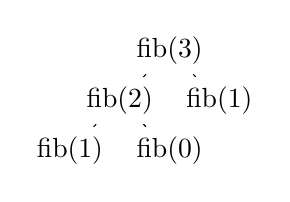
\begin{tikzpicture}
  \path [level distance=1.5pc]
  node {fib(3)}
    child [sibling distance=3pc] {node {fib(2)}
      child {node {fib(1)}}
      child {node {fib(0)}}
    }
    child [sibling distance=3pc] {node {fib(1)}}
  ;
\end{tikzpicture}
\alert{Executing fib(3)}
\end{center}
\end{frame}

\def\mynode#1{\tikz[remember picture] \node (#1) {};}
\def\fp#1{
  \node [fill,circle,inner sep=1pt] at ($(#1.north east) + (-1pc,-19pt)$)
  (#1-fp) {};}
\def\ra#1{
  \node [fill,circle,inner sep=1pt] at ($(#1.north east) + (-1pc,-6pt)$)
  (#1-ra) {};}
\def\thefp#1{
  \node [arrow box, color=white, fill=gray, arrow box arrows={east:8pt},
         anchor=east]
  at ($(#1.north west) + (0,-6pt)$) {\sffamily \bfseries FP};
}
\def\thesp#1{
  \node [arrow box, color=white, fill=gray, arrow box arrows={east:8pt},
         anchor=east]
  at ($(#1.south west) + (0,-6pt)$) {\sffamily \bfseries SP};
}

\begin{frame}[fragile]

  \begin{columns}
    \begin{column}{0.5\textwidth}
      \begin{semiverbatim}
\hlta<2,3,4,6,9>int fib(int n) \{
    int tmp1, tmp2, tmp3;
    tmp1 = n < 2;
    if (!tmp1) goto L1;
\hlta<4,6,9>    return 1;
\hlta<2,3>L1: tmp1 = n - 1;
\hlta<5,8>    tmp2 = \hlta<2,3>fib(tmp1);\mynode{pc1}
\hlta<5,8>L2: tmp1 = n - 2;
\hlta<7,10>    tmp3 = \hlta<5,8>fib(tmp1);\mynode{pc2}
\hlta<7,10>L3: tmp1 = tmp2 + tmp3;
    return tmp1;
\}
      \end{semiverbatim}
%\only<1>{1}\only<2>{2}\only<3>{3}\only<4>{4}\only<5>{5}\only<6>{6}\only<7>{7}\only<8>{8}\only<9>{9}\only<10>{10}
    \end{column}
    \begin{column}{0.5\textwidth}
      \begin{overlayarea}{\textwidth}{\textheight}
        \small
      \begin{tikzpicture}[remember picture]
        \matrix [every node/.style={draw,fill=white,drop shadow,
            text width=8pc}] {
            \node [draw=white] (s0) {n = 3}; \\
            \only<2->{
            \node (s1) {return address\\
              last frame pointer \\
              tmp1 = \only<2-7>{2}%
                     \only<8-9>{1}%
                     \only<10>{3\textcolor{red}{$\leftarrow$ result}}\\
              tmp2 = \only<8->{2}\\
              tmp3 = \only<10>{1}
              \only<2-9>{\\
              n = \only<2-7>{2}%
                  \only<8->{1}}}; }\\
            \only<3-7,9>{
            \node (s2) {return address\\
              last frame pointer \\
              tmp1 = \only<3-4,9>{1}%
                     \only<5-6>{0}%
                     \only<7>{2}\\
              tmp2 = \only<5-7>{1}\\
              tmp3 = \only<7>{1}\\
              \only<1-6>{n = \only<1-4>{1}%
                  \only<5->{0}}}; } \\
            \only<4,6>{
            \node (s3) {return address\\
              last frame pointer \\
              tmp1 = 1\\
              tmp2 = \\
              tmp3 =}; } \\
        };
        \only<1>{\thesp{s0}}
        \only<2,8,10>{\thefp{s1}\thesp{s1}}
        \only<3,5,7,9>{\thefp{s2}\thesp{s2}}
        \only<4,6>{\thefp{s3}\thesp{s3}}
        \only<2->{\fp{s1}\ra{s1}}
        \only<3-7,9>{\fp{s2}\ra{s2}}
        \only<4,6>{\fp{s3}\ra{s3}}
        \draw (s0.north west) -- (s0.south west) --
              (s0.south east) -- (s0.north east);
      \end{tikzpicture}
      \end{overlayarea}
      \begin{tikzpicture}[remember picture, overlay]
        \only<2->{
          \draw [->] (s1-fp) -| ++(3pc,4pc);
          \draw [->] (s1-ra) -- ++ (-2pc,2pc);
        }
        \only<3-7>{
          \draw [->] (s2-ra) to [out=-150,in=10] (pc1);}
        \only<9>{
          \draw [->] (s2-ra) to [out=-150,in=10] (pc2);}
        \only<3-7,9>{
          \draw [->] (s2-fp) -- ++(4pc,0) |-
                ($(s1.north east)+(0,-6pt)$);
        }
        \only<4>{\draw [->] (s3-ra) to [out=150,in=-10] (pc1);}
        \only<6>{\draw [->] (s3-ra) to [out=150,in=-10] (pc2);}
        \only<4,6>{
          \draw [->] (s3-fp) -- ++(3pc,0) |-
                ($(s2.north east)+(0,-6pt)$);
        }
      \end{tikzpicture}
    \end{column}
  \end{columns}

\end{frame}

\begin{frame}[fragile]{Allocating Fixed-Size Arrays}

Local arrays with fixed size are easy to stack.

\begin{minipage}{0.3\textwidth}
\begin{C}
void foo()
{
  int a;
  int b[10];
  int c;
}
\end{C}
\end{minipage}
%
\begin{tabular}{|c|l}
\\
\cline{1-1}
return address & $\leftarrow$ FP \\
\cline{1-1}
a \\
\cline{1-1}
b[9] \\
$\vdots$ \\
b[0] \\
\cline{1-1}
c & $\leftarrow$ FP $-$ 48 \\
\cline{1-1}
\\
\end{tabular}

\end{frame}



\begin{frame}[fragile]
  \frametitle{Allocating Variable-Sized Arrays}

Variable-sized local arrays aren't as easy.

\begin{minipage}{0.37\textwidth}
\begin{C}
void foo(int n)
{
  int a;
  int b[n];
  int c;
}
\end{C}

\end{minipage}
%
\begin{tabular}{|c|l}
\\
\cline{1-1}
return address & $\leftarrow$ FP \\
\cline{1-1}
a \\
\cline{1-1}
b[n-1] \\
$\vdots$ \\
b[0] \\
\cline{1-1}
c & $\leftarrow$ FP $-$ ? \\
\cline{1-1}
\end{tabular}

Doesn't work: generated code expects a fixed offset for c.  Even worse 
for multi-dimensional arrays.

\end{frame}

\begin{frame}[fragile]
  \frametitle{Allocating Variable-Sized Arrays}

\begin{minipage}{0.5\textwidth}
As always:\\ add a level of indirection

\medskip

\begin{C}
void foo(int n)
{
  int a;
  int b[n];
  int c;
}
\end{C}
\end{minipage}
%
\begin{tabular}{|c|@{}l}
\\
\cline{1-1}
return address & $\leftarrow$ FP \\
\cline{1-1}
a \\
\cline{1-1}
\tikz[remember picture] \node (b) {b-ptr}; \\
\cline{1-1}
c \\
\cline{1-1}
b[n-1] \\
$\vdots$ \\
\tikz[remember picture] \node (b1) {b[0]}; \\[-3pt]
\cline{1-1}
\end{tabular}

\begin{tikzpicture}[remember picture,overlay]
  \draw [->] (b) to [out=-10,in=10] (b1);
\end{tikzpicture}

Variables remain constant offset from frame pointer.

\end{frame}

%
%
%
%\begin{frame}[fragile]{Nesting Function Definitions}
%
%\begin{columns}
%  \begin{column}{0.5\textwidth}
%\shadowstart
%\begin{lstlisting}[language=caml,morendkeywords={words},ndkeywordstyle={\itshape\color{red}}]
%let articles words =
%
%  let report w =
%
%    let count = List.length
%      (List.filter ((=) w) words)
%    in w ^ ": " ^
%       string_of_int count
%
%  in String.concat ", "
%    (List.map report ["a"; "the"])
%
%in articles
%    ["the"; "plt"; "class"; "is";
%     "a"; "pain"; "in";
%     "the"; "butt"]
%\end{lstlisting}
%\shadowend
%  \end{column}
%  \begin{column}{0.5\textwidth}
%\shadowstart
%\begin{lstlisting}[language=caml,morendkeywords={words},ndkeywordstyle={\itshape\color{red}}]
%let count words w = List.length
%  (List.filter ((=) w) words) in
%
%let report words w = w ^ ": " ^
%  string_of_int (count words w) in
%
%let articles words =
%  String.concat ", "
%    (List.map (report words)
%     ["a"; "the"]) in
%
%articles
%    ["the"; "plt"; "class"; "is";
%     "a"; "pain"; "in";
%     "the"; "butt"]
%\end{lstlisting}
%\shadowend
%  \end{column}
%\end{columns}
%
%Produces ``a: 1, the: 2''
%
%\end{frame}

\def\stackframe#1#2{
 \node [frame] (#1) {(access link)\\#2}
    node [fill,circle,inner sep=1pt] at ($(#1.north east) + (-6pt,-6pt)$)
      (#1-sl) {}
    node [anchor=east] at (#1.west) {#1:};
}

\def\link#1#2{
  \draw [->] (#1-sl) to [out=45,in=-15] ($(#2.north east) + (0,-6pt)$);
}

\begin{frame}[fragile]{Implementing Nested Functions with Access Links}

\begin{columns}
  \begin{column}{0.5\textwidth}
\begin{ocaml}
let a x s =

  let b y =

    let c z = z + s in

    let d w = c (w+1) in

    d (y+1) in (* b *)

  let e q = b (q+1) in

e (x+1) (* a *)
\end{ocaml}

What does ``a 5 42'' give?

% 51

  \end{column}
  \begin{column}{0.5\textwidth}
      \begin{overlayarea}{\textwidth}{0.8\textheight}
\begin{tikzpicture}
  \matrix [frame/.style={draw,fill=white,drop shadow,text width=6pc},
           row sep=5pt] {
    \stackframe{a}{x = 5\\s = 42} \\
    \only<2->{\stackframe{e}{q = 6}} \\
    \only<3->{\stackframe{b}{y = 7}} \\
    \only<4->{\stackframe{d}{w = 8}} \\
    \only<5->{\stackframe{c}{z = 9}} \\
    };
  \only<2->{\link e a}
  \only<3->{\link b a}
  \only<4->{\link d b}
  \only<5->{\link c b}
\end{tikzpicture}
      \end{overlayarea}
  \end{column}
\end{columns}
\end{frame}

\part{In-Memory Layout Issues}


\begin{frame}[fragile]{Layout of Records and Unions}

Modern processors have byte-addressable memory.

\begin{columns}
  \begin{column}{0.1\textwidth}
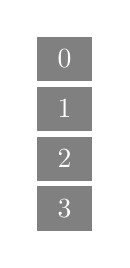
\begin{tikzpicture}
  \matrix [every node/.style=byte] {
    \node {0}; \\
    \node {1}; \\
    \node {2}; \\
    \node {3}; \\
  };
\end{tikzpicture}
  \end{column}
  \begin{column}{0.35\textwidth}
    \includegraphics[width=\textwidth]{ibm_360.jpg}
  \end{column}
  \begin{column}{0.4\textwidth}   
    \small The IBM 360 (c. 1964) helped to popularize byte-addressable memory.
  \end{column}
\end{columns}

Many data types (integers, addresses, floating-point numbers) are
wider than a byte.

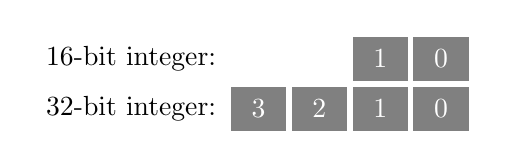
\begin{tikzpicture}
  \matrix {
    \node {16-bit integer:}; & & & \node [byte] {1}; & \node [byte] {0}; \\
    \node {32-bit integer:}; & \node [byte] {3}; & \node [byte] {2}; &
                            \node [byte] {1}; & \node [byte] {0}; \\
    };
\end{tikzpicture}

\end{frame}



\begin{frame}[fragile]{Layout of Records and Unions}

\small
\begin{columns}
  \begin{column}{0.5\textwidth}
\parskip=6pt

Modern memory systems read data in 32-, 64-, or 128-bit chunks:

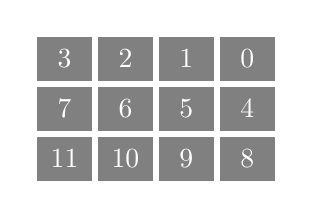
\begin{tikzpicture}
  \matrix [every node/.style=byte] {
     \node {3}; &  \node {2}; & \node {1}; & \node {0}; \\
     \node {7}; &  \node {6}; & \node {5}; & \node {4}; \\
    \node {11}; & \node {10}; & \node {9}; & \node {8}; \\
    };
\end{tikzpicture}

Reading an aligned 32-bit value is fast: a single operation.

\begin{tikzpicture}
  \matrix [every node/.style=byte] {
     \node {3}; &  \node {2}; & \node {1}; & \node {0}; \\
     \node [hbyte] {7}; & \node [hbyte] {6}; & \node [hbyte] {5}; & \node [hbyte] {4}; \\
    \node {11}; & \node {10}; & \node {9}; & \node {8}; \\
    };
\end{tikzpicture}
  \end{column}
  \begin{column}{0.5\textwidth}
\parskip=6pt

    It is harder to read an unaligned value: two reads plus shifting

\begin{tikzpicture}
  \matrix [every node/.style=byte] {
     \node [hbyte] (3) {3}; &  \node {2}; & \node {1}; & \node {0}; \\
     \node {7}; & \node [hbyte] (6) {6}; & \node [hbyte] (5) {5}; & \node [hbyte] (4) {4}; \\
    \node {11}; & \node {10}; & \node {9}; & \node {8}; \\
    \\[15pt]
     \node [hbyte] (6a) {6}; & \node [hbyte] (5a) {5}; & \node [hbyte] (4a) {4}; & \node [hbyte] (3a) {3}; \\
    };
  \draw [->] (3) edge (3a)
             (4) edge (4a)
             (5) edge (5a)
             (6) edge (6a);
\end{tikzpicture}

SPARC and ARM prohibit unaligned accesses

MIPS has special unaligned load/store instructions

x86, 68k run more slowly with unaligned accesses

  \end{column}
\end{columns}
\end{frame}

\begin{frame}[fragile]{Padding}
\small

To avoid unaligned accesses, the C compiler pads the layout of unions
and records. Rules:

\begin{itemize}
  \item Each $n$-byte object must start on a multiple of $n$ bytes (no
    unaligned accesses).

   \item Any object containing an $n$-byte object must be of size $mn$ for some
     integer $m$ (aligned even when arrayed).
\end{itemize}

\begin{columns}
\begin{column}[t]{0.5\textwidth}
\begin{C}
struct padded {
  int x;   /* 4 bytes */
  char z;  /* 1 byte  */
  short y; /* 2 bytes */
  char w;  /* 1 byte  */
};
\end{C}

\begin{tikzpicture}
  \matrix [every node/.style=hbyte] {
    \node {x}; & \node {x}; & \node {x}; & \node {x}; \\
    \node {y}; & \node {y}; & \node [byte] {}; & \node {z}; \\
    \node [byte] {}; & \node [byte] {}; & \node [byte] {}; & \node {w}; \\
    };
\end{tikzpicture}
  \end{column}
  \begin{column}[t]{0.5\textwidth}
\begin{C}
struct padded {
  char a;  /* 1 byte  */
  short b; /* 2 bytes */
  short c; /* 2 bytes */
};
\end{C}

\begin{tikzpicture}
  \matrix [every node/.style=hbyte] {
    \node {b}; & \node {b}; & \node [byte] {}; & \node {a}; \\
     & & \node {c}; & \node {c}; \\
    };
\end{tikzpicture}
  \end{column}
\end{columns}

\end{frame}


\begin{frame}[fragile]{Padding}
\small

To avoid unaligned accesses, the C compiler pads the layout of unions
and records. Rules:

\begin{itemize}
  \item Each $n$-byte object must start on a multiple of $n$ bytes (no
    unaligned accesses).

   \item Any object containing an $n$-byte object must be of size $mn$ for some
     integer $m$ (aligned even when arrayed).
\end{itemize}

\begin{columns}
\begin{column}[t]{0.5\textwidth}
\begin{C}
struct padded {
  int x;   /* 4 bytes */
  char z;  /* 1 byte  */
  char w;  /* 1 byte  */
  short y; /* 2 bytes */
};
\end{C}

\begin{tikzpicture}
  \matrix [every node/.style=hbyte] {
    \node {x}; & \node {x}; & \node {x}; & \node {x}; \\
    \node {y}; & \node {y}; & \node  {w}; & \node {z}; \\
    };
\end{tikzpicture}
  \end{column}
  \begin{column}[t]{0.5\textwidth}
\begin{C}
struct padded {
  char a;  /* 1 byte  */
  short b; /* 2 bytes */
  short c; /* 2 bytes */
};
\end{C}

\begin{tikzpicture}
  \matrix [every node/.style=hbyte] {
    \node {b}; & \node {b}; & \node [byte] {}; & \node {a}; \\
     & & \node {c}; & \node {c}; \\
    };
\end{tikzpicture}
  \end{column}
\end{columns}

\end{frame}


\begin{frame}[fragile]{Unions}
\footnotesize
A C \emph{struct} has a separate space for each field; a C
\emph{union} shares one space among all fields

\begin{columns}
  \begin{column}[t]{0.45\textwidth}
\begin{C}
union intchar {
  int i;   /* 4 bytes */
  char c;  /* 1 byte  */
};
\end{C}

\begin{tikzpicture}
  \matrix [every node/.style=hbyte] {
    \node {i}; & \node {i}; & \node {i}; & \node {i/c}; \\
    };
\end{tikzpicture}
  \end{column}
  \begin{column}[t]{0.5\textwidth}
\begin{C}
union twostructs {
  struct {
    char c;   /* 1 byte */
    int i;    /* 4 bytes */
  } a;
  struct {
    short s1; /* 2 bytes */
    short s2; /* 2 bytes */
  } b;
};
\end{C}

\begin{tikzpicture}
  \matrix [every node/.style=hbyte] at (0,2pc) {
    \node [byte] {}; &
    \node [byte] {}; &
    \node [byte] {}; &
    \node {c}; \\
    \node {i}; &
    \node {i}; &
    \node {i}; &
    \node {i}; \\
  };

\node {or};

  \matrix [every node/.style=hbyte] at (0,-2pc) {
    \node {s2}; &
    \node {s2}; &
    \node {s1}; &
    \node {s1}; \\
    \node [byte] {}; &
    \node [byte] {}; &
    \node [byte] {}; &
    \node [byte] {}; \\
  };
\end{tikzpicture}
  \end{column}
\end{columns}

\end{frame}

\begin{frame}[t,fragile]{Arrays}

\begin{columns}
  \begin{column}{0.5\textwidth}
Basic policy in C: an array is just one
object after another in memory.

\medskip

\begin{C}
int a[10];
\end{C}
  \end{column}
  \begin{column}{0.5\textwidth}
\begin{tikzpicture}
  \matrix [bytes] {
    a[0] & a[0] & a[0] & a[0] \\
    a[1] & a[1] & a[1] & a[1] \\[1.5pc]
    a[9] & a[9] & a[9] & a[9] \\
  };
\node at (0,-0.5pc) {$\vdots$};
\end{tikzpicture}
  \end{column}
\end{columns}

\vspace{1pc}

\begin{columns}
  \begin{column}{0.5\textwidth}
This is why you need padding at the end of \emph{structs}.

\medskip

\begin{C}
struct {
  int a;
  char c;
} b[2];
\end{C}
  \end{column}
  \begin{column}{0.5\textwidth}
\begin{tikzpicture}
  \matrix [bytes] (bytes) {
    a & a & a & a \\
    & & & c \\
    a & a & a & a \\
    & & & c \\
  };
\node [right] at ($(bytes.north east)!0.25!(bytes.south east)$) {b[0]};
\node [right] at ($(bytes.north east)!0.75!(bytes.south east)$) {b[1]};
\end{tikzpicture}
  \end{column}
\end{columns}

\end{frame}

\begin{frame}[fragile]{Arrays and Aggregate types}

\begin{columns}
  \begin{column}{0.5\textwidth}
The largest primitive type dictates the alignment

\medskip

\begin{C}
struct {
  short a;
  short b;
  char c;
} d[4];
\end{C}
  \end{column}
  \begin{column}{0.5\textwidth}
\begin{tikzpicture}
  \matrix [bytes] (bytes) {
    b & b & a & a \\
    a & a &   & c \\
      & c & b & b \\
    b & b & a & a \\
    a & a &   & c \\
      & c & b & b \\
  };
\node [right] at ($(bytes.north east)!0.0833!(bytes.south east)$) {d[0]};
\node [right] at ($(bytes.north east)!0.25!(bytes.south east)$) {d[1]};
\node [right] at ($(bytes.north east)!0.583!(bytes.south east)$) {d[2]};
\node [right] at ($(bytes.north east)!0.75!(bytes.south east)$) {d[3]};
\end{tikzpicture}
  \end{column}
\end{columns}

\end{frame}

\begin{frame}[fragile]{Arrays of Arrays}
\begin{columns}
  \begin{column}{0.3\textwidth}
\begin{C}
char a[4];
\end{C}
  \end{column}
  \begin{column}{0.7\textwidth}
\begin{tikzpicture}
  \matrix [bytes] (bytes) {
    a[3] & a[2] & a[1] & a[0] \\
  };
\end{tikzpicture}
  \end{column}
\end{columns}

\vspace{3pc}

\begin{columns}
  \begin{column}{0.3\textwidth}
\begin{C}
char a[3][4];
\end{C}
  \end{column}
  \begin{column}{0.7\textwidth}
\begin{tikzpicture}
  \matrix [bytes] (bytes) {
    a[0][3] & a[0][2] & a[0][1] & a[0][0] \\
    a[1][3] & a[1][2] & a[1][1] & a[1][0] \\
    a[2][3] & a[2][2] & a[2][1] & a[2][0] \\
  };
\node [right] at ($(bytes.north east)!0.166!(bytes.south east)$) {a[0]};
\node [right] at ($(bytes.north east)!0.5!(bytes.south east)$) {a[1]};
\node [right] at ($(bytes.north east)!0.833!(bytes.south east)$) {a[2]};
\end{tikzpicture}
  \end{column}
\end{columns}
\end{frame}

\part{The Heap}

\begin{frame}
  \frametitle{Heap-Allocated Storage}

Static works when you know everything beforehand and always need it.

Stack enables, but also requires, recursive behavior.

A \emph{heap} is a region of memory where blocks can be allocated and
deallocated in any order.

(These heaps are different than those in, e.g., heapsort)

\end{frame}



\begin{frame}[fragile]
  \frametitle{Dynamic Storage Allocation in C}

\shadowstart
\begin{lstlisting}[language=C,morendkeywords={malloc,free},ndkeywordstyle={\itshape\color{red}}]
struct point {
   int x, y;
};

int play_with_points(int n)
{
  int i;
  struct point *points;

  points = malloc(n * sizeof(struct point));

  for ( i = 0 ; i < n ; i++ ) {
    points[i].x = random();
    points[i].y = random();
  }

  /* do something with the array */

  free(points);
}
\end{lstlisting}
\shadowend

\end{frame}

\newlength{\unitbox}
\setlength{\unitbox}{3.5em}
\newcommand{\used}[1]{%
\tikz[baseline=-3pt] \node [used, minimum width=#1\unitbox] {};}

\newcommand{\free}[1]{%
\tikz[baseline=-3pt] \node [free, minimum width=#1\unitbox] {};}

\begin{frame}
  \frametitle{Dynamic Storage Allocation}

\parskip=1pc

\used{1}\used{2}\free{1}\used{2.5}\free{0.5}\used{0.5}\used{0.2}

\pause

\hspace{\unitbox}\hbox to 2\unitbox{\hfil $\downarrow$\rlap{ \texttt{free(\used{2})}} \hfil}

\pause

\used{1}\free{3}\used{2.5}\free{0.5}\used{0.5}\used{0.2}

\pause

\hspace{1.5\unitbox}$\downarrow$ \texttt{malloc(\used{2.5})}

\pause

\used{1}\used{2.5}\free{0.5}\used{2.5}\free{0.5}\used{0.5}\used{0.2}

\end{frame}



\begin{frame}
  \frametitle{Dynamic Storage Allocation}

Rules:

{\parindent=1em
Each allocated block contiguous (no holes)

Blocks stay fixed once allocated
}

\texttt{malloc()}

{\parindent=1em
Find an area large enough for requested block

Mark memory as allocated
}

\texttt{free()}

{\parindent=1em
Mark the block as unallocated
}

\makebox[\textwidth][r]{\raisebox{-2pc}[0pt][0pt]{%
  \includegraphics[width=10pc]{sushi-conveyor-restaurant.jpg}}}

\end{frame}


\begin{frame}
  \frametitle{Simple Dynamic Storage Allocation}

Maintaining information about free memory

{\parindent=1em
Simplest: Linked list
}

The algorithm for locating a suitable block

{\parindent=1em
Simplest: First-fit
}

The algorithm for freeing an allocated block

{\parindent=1em
Simplest: Coalesce adjacent free blocks
}

\end{frame}

\setlength{\unitbox}{1.3pc}

\begin{frame}[fragile]{Simple Dynamic Storage Allocation}

  \begin{tikzpicture}[node distance=1pc]
    \matrix (m0) {
      \node [free,minimum width=1\unitbox] {S}; &
      \node [free,minimum width=1\unitbox] (n0) {N}; &
      \node [free,minimum width=5\unitbox] {}; &
      \node [used,minimum width=1\unitbox] {S}; &
      \node [used,minimum width=2\unitbox] {}; &
      \node [free,minimum width=1\unitbox] {S}; &
      \node [free,minimum width=1\unitbox] (n1) {N}; &
      \node [free,minimum width=2\unitbox] {};
      \\
    };
    \draw [<-] (n0.north) to [out=135,in=0] ($(n0.north) + (-3pc,1pc)$);
    \draw [->] (n0.north) .. controls ($(n0.north) + (1pc,2pc)$) and
    ($(n1.north) + (-1pc,2pc)$) .. (n1.north);
    \draw [->] (n1.north) to [out=45,in=180] ($(n1.north) + (4pc,1pc)$);

    \pause

    \matrix [below=of m0] (m1) {
      \node {\ttfamily malloc(}; &
      \node [used,minimum width=3\unitbox] {}; &
      \node {\ttfamily )}; \\
    };

    \pause

    \matrix [below=of m1] (m2) {
      \node [used,minimum width=1\unitbox] {S}; &
      \node [used,minimum width=3\unitbox]  {}; &
      \node [free,minimum width=1\unitbox] {S}; &
      \node [free,minimum width=1\unitbox] (n2) {N}; &
      \node [free,minimum width=1\unitbox] {}; &
      \node [used,minimum width=1\unitbox] {S}; &
      \node [used,minimum width=2\unitbox] (u0) {}; &
      \node [free,minimum width=1\unitbox] {S}; &
      \node [free,minimum width=1\unitbox] (n3) {N}; &
      \node [free,minimum width=2\unitbox] {};
      \\
    };

    \draw [<-] (n2.north) to [out=145,in=0] ($(n2.north) + (-8pc,1pc)$);
    \draw [->] (n2.north) .. controls ($(n2.north) + (1pc,1.5pc)$) and
    ($(n3.north) + (-1pc,1.5pc)$) .. (n3.north);
    \draw [->] (n3.north) to [out=45,in=180] ($(n3.north) + (4pc,1pc)$);

    \pause

    \matrix [below=of m2] (m3) {
      \node {\ttfamily free(}; &
      \node [fill,circle,inner sep=1pt] at (0,-6pt) (p1) {}; & 
      \node {\ttfamily )}; \\
    };

    \draw [->] (p1) to [out=80,in=-100] (u0.south west);

    \pause 

    \matrix [below=of m3] (m4) {
      \node [used,minimum width=1\unitbox] {S}; &
      \node [used,minimum width=3\unitbox]  {}; &
      \node [free,minimum width=1\unitbox] {S}; &
      \node [free,minimum width=1\unitbox] (n4) {N}; &
      \node [free,minimum width=8\unitbox] {};
      \\
    };

    \draw [<-] (n4.north) to [out=145,in=0] ($(n4.north) + (-8pc,1pc)$);
    \draw [->] (n4.north) to [out=35,in=180] ($(n4.north) + (12pc,1pc)$);

  \end{tikzpicture}

\end{frame}

\begin{frame}{Dynamic Storage Allocation}

Many, many other approaches.

Other ``fit'' algorithms

Segregation of objects by size

More clever data structures

\end{frame}
%
%\begin{frame}{Heap Variants}
%
%Memory pools: Differently-managed heap areas
%
%Stack-based pool: only free whole pool at once
%
%{\parindent=1em
%Nice for build-once data structures
%}
%
%Single-size-object pool:
%
%{\parindent=1em
%Fit, allocation, etc. much faster
%
%Good for object-oriented programs
%}
%
%\end{frame}

\begin{frame}{Fragmentation}

\texttt{malloc( \used{2} )} seven times give

\used{2}\used{2}\used{2}\used{2}\used{2}\used{2}\used{2}

\medskip

\texttt{free()} four times gives

\free{2}\used{2}\free{2}\used{2}\free{2}\used{2}\free{2}

\medskip

\texttt{malloc( \used{4} )} ?

Need more memory; can't use fragmented memory.

%Hockey smile \hfill \includegraphics[width=3pc]{bobby-clarke-hockey-smile.jpg}

\begin{tabular}{cc}
  \includegraphics[height=5pc]{Zebra.jpg}
  &
  \includegraphics[height=4.5pc]{Tapir.jpg}
  \\
  Zebra
  &
  Tapir
  \\
\end{tabular}

\end{frame}

\begin{frame}[fragile]{Fragmentation and Handles}

Standard CS solution: Add another layer of indirection.

Always reference memory through ``handles.''

\begin{columns}
  \begin{column}{0.7\textwidth}
\begin{overlayarea}{\textwidth}{2pc}
\begin{tikzpicture}[node distance=2pc]

  \matrix (m0) {
  \only<1>{
    \node [free,minimum width=2\unitbox] {}; &
    \node [used,minimum width=2\unitbox] (u0) {}; &
    \node [free,minimum width=2\unitbox] {}; &
    \node [used,minimum width=2\unitbox] (u1) {}; &
    \node [free,minimum width=2\unitbox] {}; &
    \node [used,minimum width=2\unitbox] (u2) {};
  }%
  \only<2>{
    \node [used,minimum width=2\unitbox] (u0) {}; &
    \node [used,minimum width=2\unitbox] (u1) {}; &
    \node [used,minimum width=2\unitbox] (u2) {}; &
    \node [free,minimum width=6\unitbox] {};
  }%
    \\
  };

  \matrix [below=of m0.south west,anchor=base,matrix anchor=north west] (m1) {
    \node (pa) {\ttfamily *a}; &
    \node (pb) {\ttfamily *b}; &
    \node (pc) {\ttfamily *c}; &
    \node {Pointers}; \\
  };

  \matrix [below=of m1,anchor=base] (m2) {
    \node (ha) {\ttfamily **a}; &
    \node (hb) {\ttfamily **b}; &
    \node (hc) {\ttfamily **c}; &
    \node {Handles}; \\
  };

  \draw [->] (ha) -- (pa);
  \draw [->] (pa) -- (u0.south west);
  \draw [->] (hb) -- (pb);
  \draw [->] (pb) -- (u1.south west);
  \draw [->] (hc) -- (pc);
  \draw [->] (pc) -- (u2.south west);

\end{tikzpicture}
\end{overlayarea}
  \end{column}
  \begin{column}{0.3\textwidth}
    \includegraphics[width=\textwidth]{apple_1984_mac.jpg}

    \raggedright
    The original Macintosh did this to save memory.
  \end{column}
\end{columns}

\end{frame}

\part{Automatic Garbage Collection}

\begin{frame}{Automatic Garbage Collection}

Entrust the runtime system with freeing heap objects

Now common: Java, C\#, Javascript, Python, Ruby, OCaml and most
functional languages

\medskip

\begin{columns}[t]
\begin{column}{0.5\textwidth}
\parskip=0.5\baselineskip
\textbf{Advantages}

Much easier for the programmer

Greatly improves reliability: no memory leaks, double-freeing, or
other memory management errors
\end{column}
\begin{column}{0.5\textwidth}
\parskip=0.5\baselineskip
\textbf{Disadvantages}

Slower, sometimes unpredictably so

May consume more memory

\includegraphics[width=\textwidth]{garbage-truck.jpg}

\end{column}
\end{columns}

\end{frame}

\begin{frame}[fragile,t]{Reference Counting}

What and when to free? 

\begin{itemize}
\item Maintain count of references to each object
\item Free when count reaches zero
\end{itemize}

\begin{columns}[t]
\begin{column}{0.4\textwidth}
\begin{semiverbatim}
\hlta<2>let a = \hlta<1>(42, 17) in
\hlta<4>let b = \hlta<3>[a;a] in
\hlta<6>let c = \hlta<5>(1,2)::b in
\hlta<7-10>b
\end{semiverbatim}
\end{column}
\begin{column}{0.6\textwidth}
\ttfamily

\begin{tikzpicture}[cell/.style={rectangle split,
      rectangle split horizontal, fill=white, draw,
      anchor=west}]
\fill [color=mBlue!30] (-6pc,2.5pc) rectangle (9pc,-10pc);
\node [cell, rectangle split parts=2]
      (aa) {\only<1>{0}%
            \only<2>{1}%
            \only<3-6>{3}%
            \only<7->{2}%
            \nodepart{two} 42, 17};
\only<2-6>{
  \node (a) at ($(aa) + (-3pc, 2pc)$) {a};
  \draw [->] (a) to [bend left] (aa);
}
\only<3->{
  \node [cell, rectangle split parts=3] (bb)
      at ($(aa.west) + (down:3pc)$)
      {\only<3>{0}%
       \only<4,9->{1}%
       \only<5-8>{2}%
       \nodepart{two} \nodepart{three}};
  \node [cell, rectangle split parts=3] (bbb)
      at ($(bb.east) + (right:2pc)$)
      {1 \nodepart{two} \nodepart{three}};
  \draw [->] (bb.two) to (aa);
  \draw [->] (bb.three) to (bbb);
  \draw [->] (bbb.two) to [bend right] (aa);
  \draw [-open triangle 90] (bbb.three) -| ++(1pc,-1pc);
}
\only<4-10>{
  \node (b) at ($(bb) + (-2pc,1.5pc)$) {b};
  \draw [->] (b) to [bend left] (bb);
}
\only<5-9>{
  \node [cell, rectangle split parts=2] (ccc) at ($(bb.west) + (-5pc,-3pc)$) 
        {\only<5-8>{1}%
         \only<9>{0}%
         \nodepart{two} 1, 2};
}
\only<5-8>{
  \node [cell, rectangle split parts=3] (cc) at ($(bb) + (-6pc,0)$)
        {\only<5,8>{0}%
         \only<6-7>{1}%
         \nodepart{two} \nodepart{three}};
  \draw [->] (cc.two) to (ccc);
  \draw [->] (cc.three) to (bb);
}
\only<6-7>{
  \node (c) at ($(cc) + (-1pc,2pc)$) {c};
  \draw [->] (c) to [bend left] (cc);
}
\end{tikzpicture}

\end{column}
\end{columns}

\end{frame}

\begin{frame}{Issues with Reference Counting}

Circular structures defy reference counting:

\begin{tikzpicture}
  \node [draw] (a) {a};
  \node [draw,right=of a] (b) {b};
  \draw [->] (a) edge [bend left] (b);
  \draw [->] (b) edge [bend left] (a);
\end{tikzpicture}

Neither is reachable, yet both have non-zero reference counts.

High overhead (must update counts constantly), although incremental

\end{frame}

\begin{frame}[fragile,t]{Mark-and-Sweep}

What and when to free?

\begin{itemize}
\item Stop-the-world algorithm invoked when memory full
\item Breadth-first-search marks all reachable memory
\item All unmarked items freed
\end{itemize}

\begin{columns}[t]
\begin{column}{0.4\textwidth}
\begin{semiverbatim}
let a = (42, 17) in
let b = [a;a] in
let c = (1,2)::b in
b
\end{semiverbatim}
\end{column}
\begin{column}{0.6\textwidth}
\ttfamily

\begin{tikzpicture}[cell/.style={rectangle split,
      rectangle split horizontal, fill=white, draw,
      anchor=west}]
\fill [color=mBlue!30] (-6pc,2.5pc) rectangle (9pc,-10pc);
\only<1-4>{
\node [cell, rectangle split parts=2]
      (aa) {\only<3>{$\bullet$}
            \nodepart{two} 42, 17};
}
\only<1>{
  \node (a) at ($(aa) + (-3pc, 2pc)$) {a};
  \draw [->] (a) to [bend left] (aa);
}
  \node [cell, rectangle split parts=3] (bb)
      at ($(aa.west) + (down:3pc)$)
      {\only<2-3>{$\bullet$}\nodepart{two} \nodepart{three}};
  \node [cell, rectangle split parts=3] (bbb)
      at ($(bb.east) + (right:2pc)$)
      { \only<3>{$\bullet$}\nodepart{two} \nodepart{three}};
  \draw [->] (bb.two) to (aa);
  \draw [->] (bb.three) to (bbb);
  \draw [->] (bbb.two) to [bend right] (aa);
  \draw [-open triangle 90] (bbb.three) -| ++(1pc,-1pc);
  \node (b) at ($(bb) + (-2pc,1.5pc)$) {b};
  \draw [->] (b) to [bend left] (bb);
\only<1-3>{
  \node [cell, rectangle split parts=2] (ccc) at ($(bb.west) + (-5pc,-3pc)$) 
        {\nodepart{two} 1, 2};
  \node [cell, rectangle split parts=3] (cc) at ($(bb) + (-6pc,0)$)
        {\nodepart{two} \nodepart{three}};
  \draw [->] (cc.two) to (ccc);
  \draw [->] (cc.three) to (bb);
}
\only<1>{
  \node (c) at ($(cc) + (-1pc,2pc)$) {c};
  \draw [->] (c) to [bend left] (cc);
}
\end{tikzpicture}

\end{column}
\end{columns}

\end{frame}

\begin{frame}{Mark-and-Sweep}
\parskip=0.5\baselineskip

Mark-and-sweep is faster overall; may induce big pauses

Mark-and-compact variant also moves or copies reachable objects to
eliminate fragmentation

Incremental garbage collectors try to avoid doing everything at once

Most objects die young; generational garbage collectors segregate heap
objects by age

Parallel garbage collection tricky

Real-time garbage collection tricky

\end{frame}
%
%\part{Shared Libraries and Dynamic Linking}
%\begin{frame}
%  \frametitle{Shared Libraries and Dynamic Linking}
%
%The 1980s GUI/WIMP revolution required many large libraries
%(the Athena widgets, Motif, etc.)
%
%Under a \emph{static linking} model, each executable using a library
%gets a copy of that library's code.
%
%Address 0:
%\begin{tabular}[b]{|c|}
%\hline
%libXaw.a \\
%\hline
%libX11.a \\
%\hline
%xeyes \\
%\hline
%\end{tabular}
%\begin{tabular}[b]{|c|}
%\hline
%libXaw.a \\
%\hline
%libX11.a \\
%\hline
%xterm \\[3pc]
%\hline
%\end{tabular}
%\begin{tabular}[b]{|c|}
%\hline
%libXaw.a \\
%\hline
%libX11.a \\
%\hline
%xclock \\[5pt]
%\hline
%\end{tabular}
%
%\pause
%
%Wasteful: running many GUI programs at once fills memory with
%\hlt{nearly identical} copies of each library.
%
%Something had to be done: another level of indirection.
%
%\end{frame}
%
%\begin{frame}
%  \frametitle{Shared Libraries: First Attempt}
%\small
%Most code makes assumptions about its location.
%
%First solution (early Unix System V R3) required each shared library
%to be located at a unique address:
%
%Address 0:
%\begin{tabular}[b]{|c|@{}c@{\hspace{2pt}}|c|@{}c@{\hspace{2pt}}|c|}
%\cline{1-1}\cline{3-3}\cline{5-5}
% && && libXm.so \\[1pc]
%\cline{1-1}\cline{3-3}\cline{5-5}
%libXaw.so && libXaw.so && \\
%\cline{1-1}\cline{3-3}\cline{5-5}
%libX11.so && libX11.so && libX11.so \\
%\cline{1-1}\cline{3-3}\cline{5-5}
%\multicolumn{1}{c}{}\\[-5pt]
%\cline{5-5}
%\multicolumn{4}{c|}{} & netscape \\
%\cline{3-3}
%\multicolumn{2}{c|}{} & xterm && \\
%\cline{1-1}
%xeyes && && \\
%\cline{1-1}\cline{3-3}\cline{5-5}
%\end{tabular}
%
%\pause
%
%Obvious disadvantage: must ensure each new shared library located at a
%new address.
%
%Works fine if there are only a few libraries; tended to discourage
%their use.
%
%\end{frame}
%
%\begin{frame}
%  \frametitle{Shared Libraries}
%
%Problem fundamentally is that each program may need to see different
%libraries \hlt{each at a different address}.
%
%\begin{tabular}[b]{|c|}
%\hline
%libXaw.so \\
%\hline
%libX11.so \\
%\hline
%\multicolumn{1}{c}{}\\
%\hline
%xeyes \\
%\hline
%\end{tabular}
%%
%\begin{tabular}[b]{|c|}
%\hline
%libXaw.so \\
%\hline
%libX11.so \\
%\hline
%\multicolumn{1}{c}{}\\
%\hline
%xterm \\[2pc]
%\hline
%\end{tabular}
%%
%\begin{tabular}[b]{|c|}
%\hline
%libXm.so \\[0.5pc]
%\hline
%libX11.so \\ 
%\hline
%\multicolumn{1}{c}{}\\
%\hline
%netscape \\[3pc]
%\hline
%\end{tabular}
%
%\end{frame}
%
%\begin{frame}
%  \frametitle{Position-Independent Code}
%
%Solution: Require the code for libraries to be
%position-independent. \hlt{Make it so they can run anywhere in
%memory.}
%
%As always, add another level of indirection:
%
%\begin{itemize}
%\item All branching is PC-relative
%
%\item All data must be addressed relative to a base register.
%
%\item All branching to and from this code must go through a jump table.
%\end{itemize}
%
%\end{frame}
%
%\begin{frame}[fragile]
%  \frametitle{Position-Independent Code for bar()}
%
%  \begin{columns}
%    \begin{column}[b]{0.3\textwidth}
%\hlt{Normal unlinked code}
%
%\fontsize{8}{8}\selectfont
%\begin{semiverbatim}
%save  %sp, -112, %sp
%sethi  %hi(0), %o0
%  \hlt{R_SPARC_HI22 .bss}
%mov  %o0, %o0
%  \hlt{R_SPARC_LO10 .bss}
%sethi  %hi(0), %o1
%  \hlt{R_SPARC_HI22 a}
%mov  %o1, %o1
%  \hlt{R_SPARC_LO10 a}
%call  14
%  \hlt{R_SPARC_WDISP30 strcpy}
%nop 
%sethi  %hi(0), %o0
%  \hlt{R_SPARC_HI22 .bss}
%mov  %o0, %o0
%  \hlt{R_SPARC_LO10 .bss}
%call  24
%  \hlt{R_SPARC_WDISP30 baz}
%nop 
%ret 
%restore 
%\end{semiverbatim}
%    \end{column}
%    \begin{column}[b]{0.5\textwidth}
%\hlt{gcc -fpic -shared}
%\fontsize{8}{8}\selectfont
%\begin{semiverbatim}
%save  %sp, -112, %sp
%sethi  %hi(0x10000), %l7
%call  8e0   \hlt{! add PC to %l7}
%add  %l7, 0x198, %l7
%ld  [ %l7 + 0x20 ], %o0
%ld  [ %l7 + 0x24 ], %o1
%
%
%
%call  10a24\lab{0.5pc}{1.5pc}{Actually just a stub} ! strcpy
%
%nop 
%ld  [ %l7 + 0x20 ], %o0
%
%
%
%call\lab{0.5pc}{1.5pc}{call is PC-relative}  10a3c ! baz
%
%nop 
%ret 
%restore
%\end{semiverbatim}
%  \end{column}
%  \end{columns}
%
%\end{frame}

% \fi % FIXME

%\part{Objects and Inheritance}
%
%\begin{frame}[fragile]{Single Inheritance}
%
%Simple: Add new fields to end of the object
%
%Fields in base class always at same offset in derived class (compiler
%never reorders)
%
%Consequence: Derived classes can never remove fields
%
%%\vskip 2\baselineskip
%
%\begin{columns}
%\begin{column}[t]{0.5\textwidth}
%\textbf{C++}
%
%\begin{cpp}
%class Shape {
%  double x, y;
%};
%
%class Box : Shape {
%  double h, w;
%};
%
%
%class Circle : Shape {
%  double r;
%};
%
%\end{cpp}
%\end{column}
%\begin{column}[t]{0.5\textwidth}
%\textbf{Equivalent C}
%
%\begin{C}
%struct Shape {
%  double x, y;
%};
%
%struct Box {
%  double x, y;
%  double h, w;
%};
%
%struct Circle {
%  double x, y;
%  double r;
%};
%\end{C}
%\end{column}
%\end{columns}
%\end{frame}
%
%\begin{frame}[fragile]{Virtual Functions}
%
%\begin{cpp}
%class Shape {
%  virtual void draw(); // Invoked by object's run-time class
%};                     // not its compile-time type.
%
%class Line : public Shape {
%  void draw();
%}
%
%class Arc : public Shape {
%  void draw();
%};
%
%Shape *s[10];
%s[0] = new Line;
%s[1] = new Arc;
%s[0]->draw();   // Invoke Line::draw()
%s[1]->draw();   // Invoke Arc::draw()
%\end{cpp}
%
%\end{frame}
%
%\begin{frame}[fragile]{Virtual Functions}
%
%Trick: add to each object a pointer to the virtual table for its type,
%filled with pointers to the virtual functions.
%
%Like the objects themselves, the virtual table for each derived type
%begins identically.
%
%\begin{columns}
%\begin{column}{0.5\textwidth}
%\begin{cpp}
%struct A {
%  int x;
%  virtual void Foo();
%  virtual void Bar();
%};
%
%struct B : A {
%  int y;
%  virtual void Foo();
%  virtual void Baz();
%};
%
%A a1;
%A a2;
%B b1;
%\end{cpp}
%\end{column}
%\begin{column}{0.5\textwidth}
%\begin{tikzpicture}[%
%  show background rectangle,
%  background rectangle/.style={fill, color=mBlue!30},
%  object/.style={rectangle split,
%                 fill=white,
%                 draw
%  }
%]
%\node [object, rectangle split parts=2] (Avtbl) {
%   A::Foo
%   \nodepart{two} A::Bar
%   };
%\node [above] at (Avtbl.north) {A's Vtbl};
%\node [object, rectangle split parts=3, anchor=north] (Bvtbl)
%   at ($(Avtbl.north) + (right:6pc)$) {
%   B::Foo
%   \nodepart{two} A::Bar
%   \nodepart{three} B::Baz
%   };
%\node [above] at (Bvtbl.north) {B's Vtbl};
%
%\node [object, rectangle split parts=2, anchor=north] (a1)
%   at ($(Avtbl.south) + (down:2pc)$) { vptr
%    \nodepart{second} x};
%\node [above] at (a1.north) {a1};
%\draw [->] (a1.text east) to [bend right] (Avtbl.text east);
%
%\node [object, rectangle split parts=2, anchor=north] (a2)
%   at ($(a1.south) + (down:2pc)$) { vptr
%    \nodepart{second} x};
%\node [above] at (a2.north) {a2};
%\draw [->] (a2.text east) to [bend right] (Avtbl.text east);
%
%\node [object, rectangle split parts=3, anchor=north] (b1)
%   at ($(Bvtbl.south) + (down:2pc)$) { vptr
%    \nodepart{second} x
%    \nodepart{third} y
%    };
%\node [above] at (b1.north) {b1};
%\draw [->] (b1.text east) to [bend right] (Bvtbl.text east);
%
%
%   
%\end{tikzpicture}
%\end{column}
%\end{columns}
%
%\end{frame}

%\part{Exceptions}
%
%
%\def\mynode#1#2{\tikz[remember picture,baseline]\node[inner sep=0pt,anchor=base] (#1) {#2};}
%
%\begin{frame}[fragile]{C++'s Exceptions}
%
%\lstset{escapechar=\^}
%\begin{cpp}
%struct Except {} ex;  // This struct functions as an exception
%
%void top(void) {
%  try {
%    ^\mynode{a}{child}^();
%  } ^\mynode{f}{\bfseries catch}^ (Except e) { // throw sends control here
%    printf("oops\n");
%  }
%}
%
%void ^\mynode{b}{child}^() {
%  ^\mynode{c}{child2}^();
%}
%
%void ^\mynode{d}{child2}^() {
%  ^\mynode{e}{\textbf{throw} ex;}^ // Pass control up to the catch block
%}
%\end{cpp}
%
%\begin{tikzpicture}[remember picture,overlay]
%\begin{scope}[very thick, red, ->, font={\scriptsize},
%              every node/.style={inner sep=2pt,draw,fill=white}]
%\draw (a.south west) to [bend right=20] node [pos=0.7] {1} (b.north west);
%\draw (c) to node [pos=0.35] {2} (d);
%\draw [blue] (e.north east) to [bend right=55,looseness=1.5]
%                            node [pos=0.25] {3} (f.south east);
%\end{scope}
%\end{tikzpicture}
%
%\end{frame}
%
%\begin{frame}[fragile]{C's setjmp/longjmp: Idiosyncratic Exceptions}
%
%\vskip0.5\baselineskip
%
%\lstset{escapechar=\^}
%\begin{C}
%#include <setjmp.h>
%
%jmp_buf closure;          /* return address, stack & frame ptrs. */
%
%void top(void) {
%  switch ( ^\mynode{a}{setjmp}^(closure) ) { /* normal: store closure, return 0 */
%                               /* longjmp jumps here, returns 1 */
%
%
%  case 0: ^\mynode{b}{child}^();             /* unexceptional case */
%          break;
%
%  case 1: ^\mynode{e}{\bfseries break}^;               /* longjmp( ,1) called */
%  }
%}
%
%void child() {
%  ^\mynode{c}{child2}^();
%}
%
%void child2() {
%  ^\mynode{d}{longjmp(closure, 1)}^;
%}
%\end{C}
%
%\begin{tikzpicture}[remember picture,overlay]
%\begin{scope}[very thick, red, ->, font={\scriptsize},
%              every node/.style={inner sep=2pt,draw,fill=white}]
%\draw (a.south) to node [pos=0.3] {1} (b.north);
%\draw (b.south west) to [bend right=20] node [pos=0.15] {2} (c);
%\draw (c) to node [pos=0.4] {3} ($(d.north west) + (right:1pc)$);
%\draw [blue] (d.north east) to [bend right=60] node [pos=0.25] {4} (a.south east);
%\draw [blue] (a.south east) to [bend left=45] node [pos=0.25] {5} (e.north east);
%\end{scope}
%\end{tikzpicture}
%
%\end{frame}
%
%\begin{frame}[fragile]{Implementing Exceptions}
%
%One way: maintain a stack of exception handlers
%
%\begin{columns}
%\begin{column}{0.25\textwidth}
%\begin{cpp}
%try {
%
%  child();
%
%
%} catch (Ex e) {
%  foo();
%}
%
%void child() {
%  child2();
%}
%
%void child2() {
%  throw ex;
%}
%\end{cpp}
%\end{column}
%\begin{column}{0.75\textwidth}
%\begin{cpp}
%  push(Ex, Handler); // Push handler on stack
%
%  child();
%  pop();             // Normal termination
%  goto Exit;         // Jump over "catch"
%Handler:
%  foo();             // Body of "catch"
%Exit:
%
%void child() {
%  child2();
%}
%
%void child2() {
%  throw(ex);       // Unroll stack; find handler
%}
%\end{cpp}
%\end{column}
%\end{columns}
%
%Incurs overhead, even when no exceptions thrown
%\end{frame}
%
%\begin{frame}[fragile]{Implementing Exceptions with Tables}
%
%Q: When an exception is \emph{throw}n, where was the last \emph{try}?
%
%A: Consult a table: relevant handler or ``pop'' for every PC
%
%\begin{columns}
%\begin{column}{0.4\textwidth}
%\lstset{numbers=left,escapechar=\^}
%\begin{cpp}
%void foo() {
%
%  try {
%    ^\mynode{e}{bar();}^
%  } catch (Ex1 e) {
%    ^\mynode{g}{a();}^
%  }
%}
%
%void bar() {
%  ^\mynode{c}{baz();}^
%}
%
%void baz() {
%
%  try {
%    ^\mynode{a}{\textbf{throw} ex1;}^
%  } catch (Ex2 e) {
%    b();
%  }
%}
%\end{cpp}
%\end{column}
%\begin{column}{0.5\textwidth}
%%\renewcommand\arraystretch{2.3}
%\begin{tabular}{rl}
%\toprule
%\textbf{Lines} & \textbf{Action} \\
%\midrule
%1--2 & Pop stack \\
%\mynode{f}{3--5} & Handler @ 5 for Ex1 \\
%\\
%\\
%\\
%\mynode{d}{6--15} & Pop stack \\
%\\
%\\
%\\
%\mynode{b}{16--18} & Handler @ 18 for Ex2\\
%\\
%19--21 & Pop stack \\
%\bottomrule
%\end{tabular}
%
%\end{column}
%\end{columns}
%
%\begin{tikzpicture}[remember picture,overlay]
%\begin{scope}[very thick, red, ->, font={\scriptsize},
%              every node/.style={inner sep=2pt,draw,fill=white}]
%\draw (a.east) to node {1: query} (b.west);
%\draw (b.west) to node [pos=0.4] {2: pop stack} (c.east);
%\draw (c.east) to node {3: query} (d.west);
%\draw (d.west) to node [pos=0.25] {4: pop stack} (e.east);
%\draw (e.east) to [bend left=20] node {5: query} (f.west);
%\draw (f.west) to node [pos=0.35] {6: handle} (g.east);
%\end{scope}
%\end{tikzpicture}
%\end{frame}


% FIXME

% Continuations, Closures, etc.

% OCaml example that shows you need access to other values

% Idea is that ``f'' must capture the environment in which it is defined,
% Not where it is first referred to or used

\if 0
\part{Binding Reference Environments}
\frame{\partpage

\centerline{What happens when you take a snapshot of a subroutine?}
}

\begin{frame}[fragile,singleslide]{
  \frametitle{References to Subroutines}

In many languages, you can create a reference to a subroutine and call
it later.  E.g., in C,

\begin{C}
int foo(int x, int y) { /* ... */ }

void bar()
{
  int (*f)(int, int) = foo;

  (*f)(2, 3); /* invoke foo */
}
\end{C}

\end{frame}

\begin{frame}{Reference Environments: Closures}

Closure = Code + Environment

Environment = Values of non-local variables

C doesn't need closures: C functions only need access to global
variables, which are always in the same place.

\end{frame}

\begin{frame}[fragile,singleslide]
  \frametitle{References to Subroutines}

C is simple: no function nesting; only environment is the omnipresent
global one.  But what if there were?

\begin{C}
typedef int (*ifunc)();

ifunc foo() {
  int a = 1;

  int bar() { return a; } /* this is not C */

  return bar;
}

int main() {
  ifunc f = foo();  /* returns bar */
  return (*f)();    /* call bar. a? */
}
\end{C}

\end{frame}

\fi

\end{document}
